
\chapter{Overview of Documentation Platforms  and a Case Study: Instructables}
\todo{History of platform}
\todo{Timline of different platform}
\todo{properties}
\todo{case study instructable}
\todo{case study BIP}
\todo{text}
\section{Introduction}
In the maker - movement \cite{davies2017hackerspaces}, people need online tools to exchange knowledge, share experiences and to work in interdisciplinary teams to \textit{innovate}, \textit{design} and \textit{implement solutions}.

The method of online documentation has a strong influence on how useful, learnable, available, shareable and accessible results are \cite{harcourt2016re}.

\todo{add my story}
The complexity of documentation has led makers to create a variety of online communities and to experiment with different ways of documenting their results. Because documentation is often seen as tedious and time-consuming, makers are constantly seeking optimal solutions to reduce the effort needed to document their results. On the other hand, careful documentation enables makers to collaborate and share their efforts more effectively.


In this state-of-the-art, we will briefly survey a range of platforms developed to support makers in documenting their projects. We then analyse in more detail the pros and cons of two platforms, \textit{Instructables} and Build-in-Progress. In both case we discuss how authors and readers benefit from online documentation, what motivates them to share a project and – in the case of \textit{Build-in-Progress} what are the consequences of sharing a work in progress with online community.

The first part of this state-of-the-art will review \textit{Instructables}, describe how the platform works and describe in details the design orientation process. The second part will review the design approach of \textit{SDG-in-Progress} and the added features. The last part will review the user interaction of \textit{BiP}. 



\section{Instructable}


\begin{center}
	\begin{minipage}{.7\textwidth}
		\textit{In this section, I share with you an analyses of how users create and share \textit{DIY} projects via online platform called Instructables. I share findings of the analyses of this platform and the understanding of how authors and users use Instructables}
	\end{minipage}
\end{center}

\begin{comment}
\hl{What is it ?} \hl{Who use it ?} \hl{User interactions ?} \hl{Limitations} \hl{Advantages ?} \hl{Examples ?} \\
\end{comment}

\begin{figure}[ht!]
	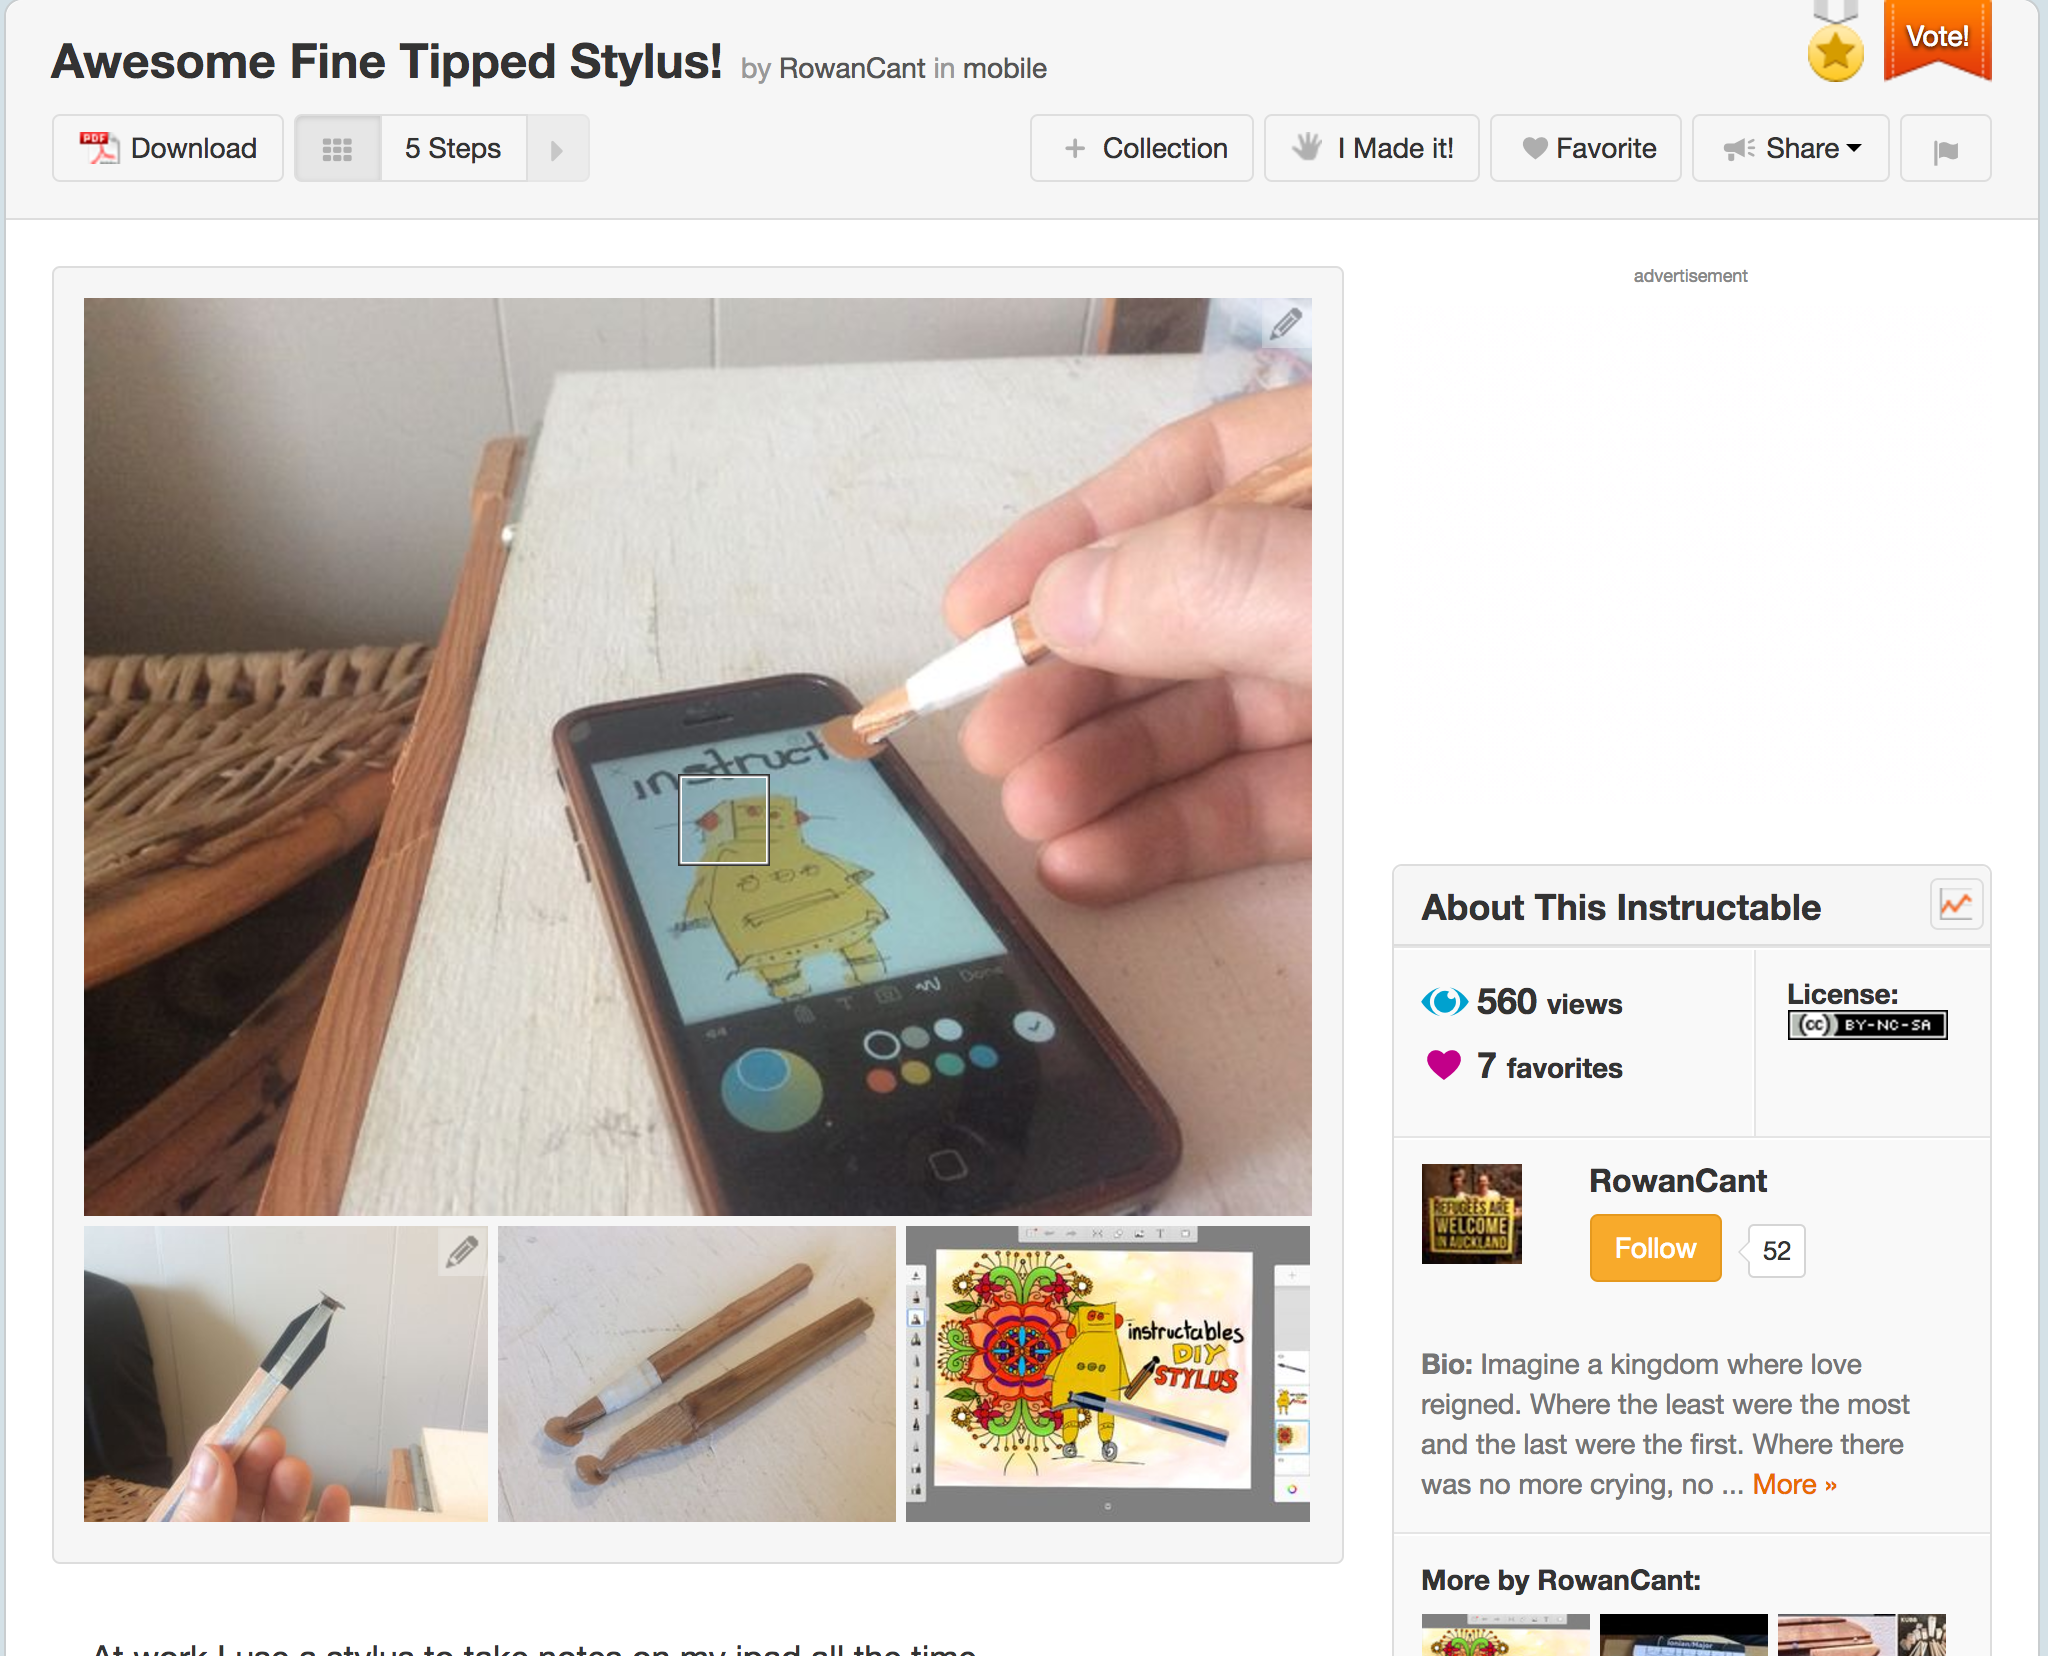
\includegraphics[scale=0.36]{./images/img-instructables.png}
	\caption{Sample Instructables project, \url{http://www.instructables.com/id/Awesome-Fine-Tipped-Stylus/}}
	\label{sec:img-instructables}
\end{figure}

Instructables is an online platform for \textit{DIY} communities that serves as a "place that lets you explore, document, and share your creations" \cite{web:instructable}. It is a website specializing in user-created and uploaded do-it-yourself projects, which other users can comment on and rate for quality \cite{wiki:instructable} \cite{wiki:instructable}. There are different categories of project such as technology, crafts, food, home, workshops and living, with more than 263,258 projects and 9,888,442 monthly visit as of August 2017. Users create their project step by step and with each step they describe what they did in a text, photos or videos as displayed in the figure \ref{sec:img-instructables}. The encapsulation of steps produce a typical guide that help others to re-create the project, learn from it or build a new thing on top of it and have their own version of the project. 

The contributions in Instructables come from the sharing culture of projects, not only authors contribute but also readers who can view and give feedback by commenting on the project. Also, Instructables create a social community where they exchange their thoughts about a topic via forums and subforms dedicated to a special topic such as Arduino projects. Finally, prizes are given to the top shared Instructables as a kind of reward for their effort of sharing their project and to keep them connected with the community.

\subsection{Methodology} 

To understand the users interactions of Instructables, an extensive study of the Instructables community has been done in the fall of 2011, this study used semi-structured interviews and online surveys. The semi-structured interviews had a framework of four themes that had been explored : (\oldstylenums{1}) motivation, (\oldstylenums{2}) Documentation tools, (\oldstylenums{3}) Writing an Instructable and (\oldstylenums{4}) Feedback. A theme was covered by a set of questions that took one hour with each interviewer. \cite{scholar:Tseng:2014:PVP:2598510.2598540}. A survey of 15 multiple-choice questions and open ended-questions that ask users about different aspects of their experience with replicating or building on top of a project shared by a user on the platform.

\subsection{User interaction}

The study has shown three strategies for documenting a project. The first was to \textit{write after you make}, as shown in the figure \ref{img-writemake}  \cite{tseng2016making}.
\begin{figure}[ht!]
	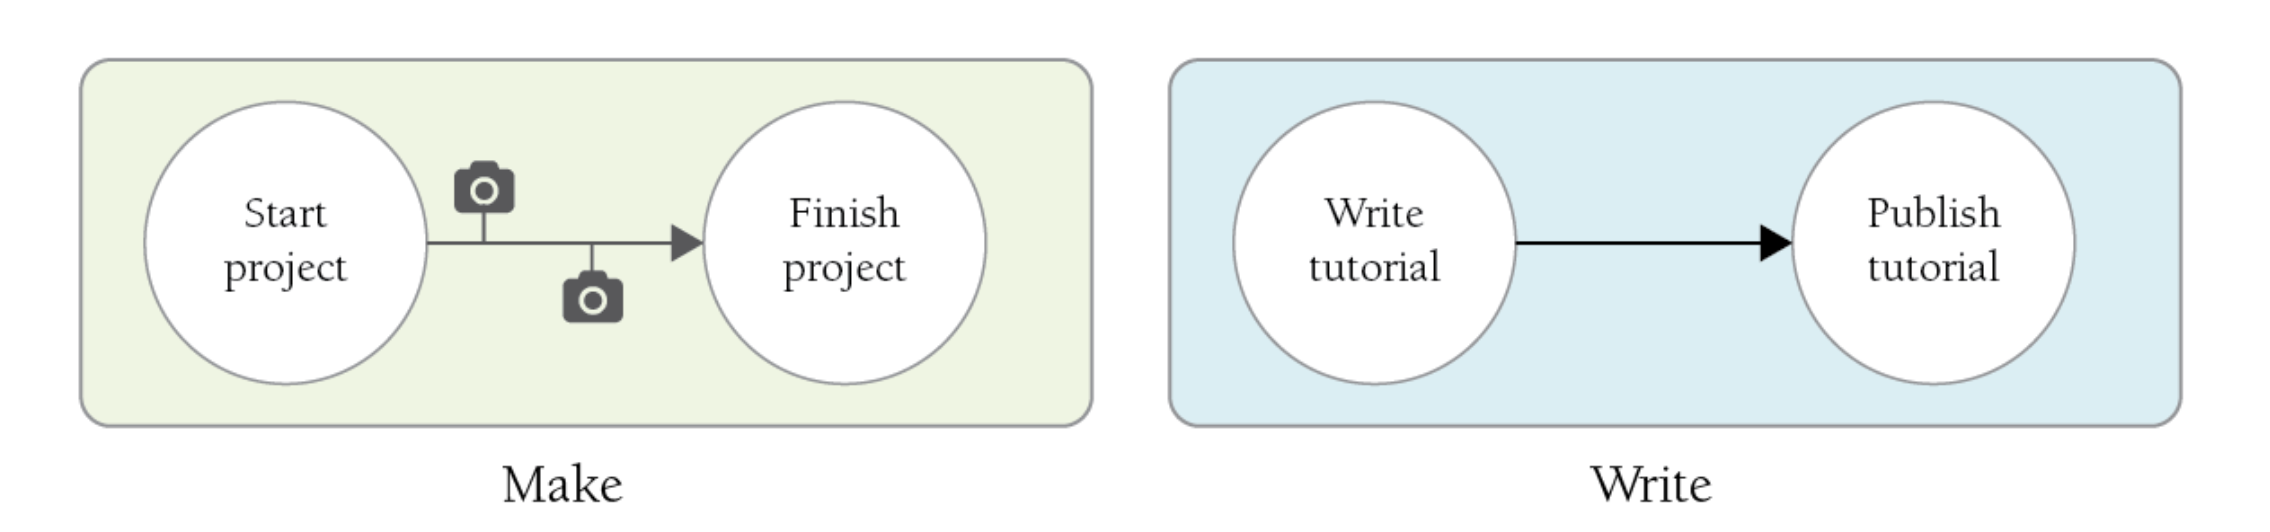
\includegraphics[scale=0.34]{./images/img-writemake.png}
	\caption{First strategy of documenting : write after you make, \cite{tseng2016making}}
	\label{img-writemake}
\end{figure}

A problem confronted the users with this strategy, users forgot to document in the midst of making. Users outperformed this problem by following the second strategy of \textit{writing after replicating}, as displayed in the figure \ref{img-makereplicatewrite} \cite{scholar:Tseng:2014:PVP:2598510.2598540}
\begin{figure}[ht!]
	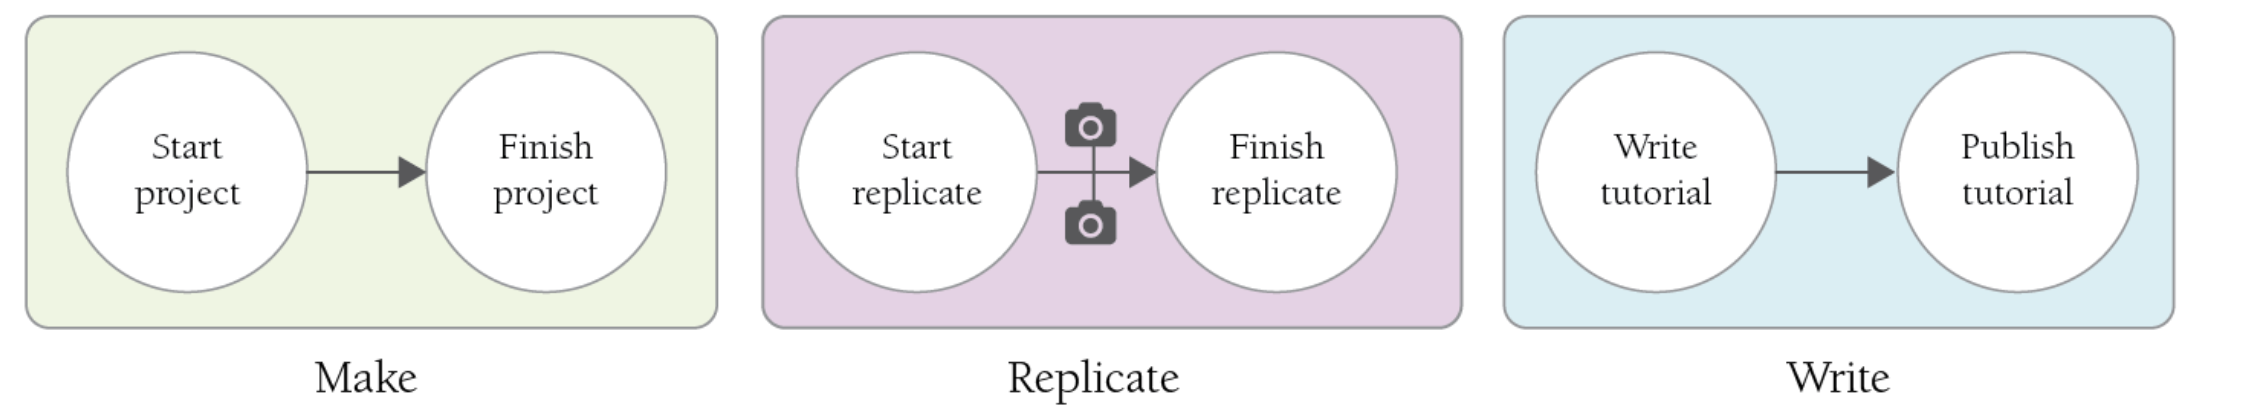
\includegraphics[scale=0.34]{./images/img-makereplicatewrite.png}
	\caption{First strategy of documenting : Make, replicate  then write, \cite{tseng2016making}}
	\label{img-makereplicatewrite}
\end{figure}

The final strategy was to \textit{simultaneously write and make} (figure \ref{img-makewritesimultanously}). 
\begin{figure}[ht!]
	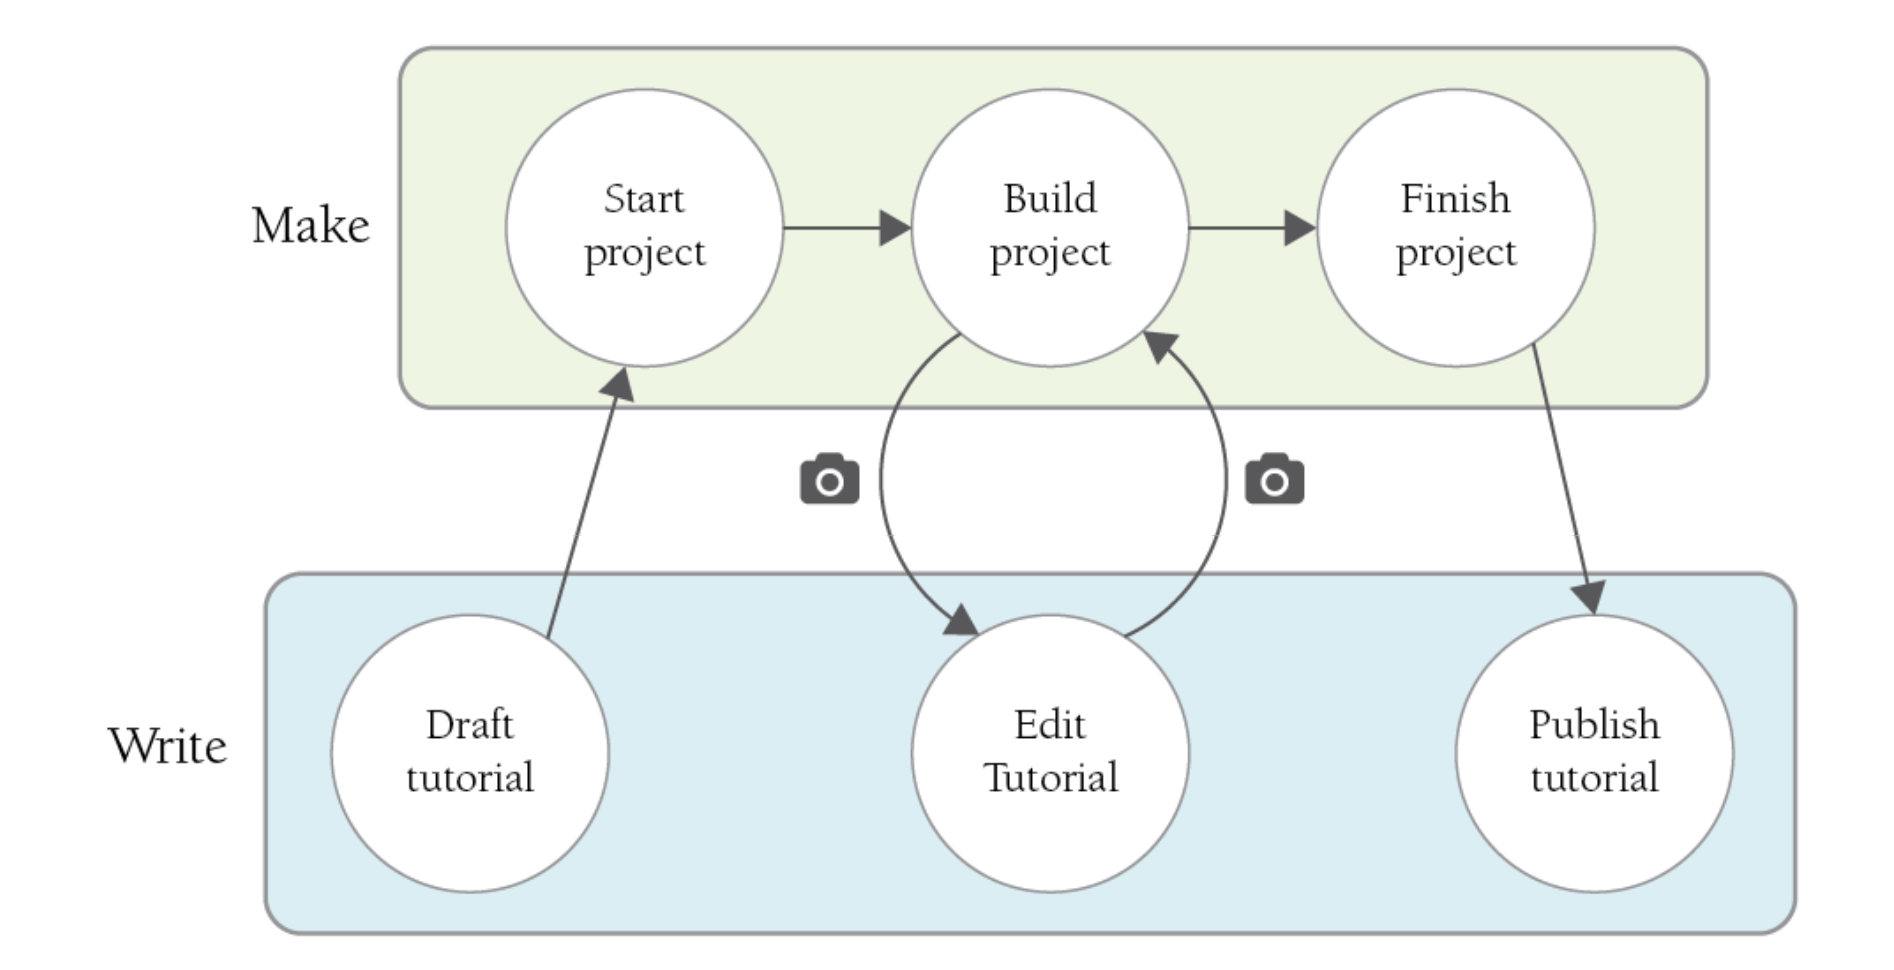
\includegraphics[scale=0.34]{./images/img-makewritesimultanously}
	\caption{First strategy of documenting : write after you make, \cite{tseng2016making}}
	\label{img-makewritesimultanously}
\end{figure}

In summary, the study showed that users need to encapsulate the collected photos and videos to show to create all the steps and a common challenge was to remember to document after each step otherwise users had to replicate their project merely to creating good documentation. 

Finally, authors saw that documentation well worth the effort to share their work but it is time consuming process when a project get more complex, it is hard to follow up or complete the documentation. \cite{scholar:Wakkary:2015:TAH:2702123.2702550}

\subsection{Design and process oriented documentation}
Several approaches were suggested by to improve the online documentation. Documentation techniques requires authors to simultaneously switch between making and writing, make a design process to not miss a step from not being documented or to radically recreate the project to document it in a proper way. Another challenges of documentation technique that needed to support not only the capture of digital artifacts but also physical artifacts where it is not possible to show the physical effort. 
With the recurring need to balance manual and automated ways of capturing, software and hardware tools need to solve open questions and be customizable for different activities and different audiences \cite{Kuznetsov:2010:REA:1868914.1868950}. The workflow of documentation over time needed to not miss a key step in the documentation. 

Documentation process seems to be more important for readers as it give them the opportunity to enable better decision making about components or materials to use \cite{scholar:sf1241364}, as well as successful in encouraging independent exploration and fostering a sense of accomplishment \cite{scholar:lovell2010sewing}. Also, as many users start by replicating some projects, having tools where they could be able to contribute to a project, can help more socializing and boost a collaborative work in the community. 



\begin{comment}

\begin{itemize}
	\item{Adapt  SDG in progress}
	
	
	\item{Qu-est ce que la platforme a apporte et ce que nous on a apporte}
	\item{Comparaison avec other platform}
	\item{ Explication about the summer school, experience, different way to document etc..} 
	\item{When we can use it and how we can use it ?} 
	
\end{itemize}


\begin{itemize}
	\item Platforme pour le soutien des hackathon grise
	\item What tiffanz said about here ieda and references
	\item securite constructif
	
	\begin{itemize}
		\item la continuite des  idess
		\item durabilitz of projects
		\item relance les projet
	\end{itemize}
	\item hackathons
	\item summer school
	\item master
	\item how to evaluate a project in time when it avaluate from team to team
	\item changement de step ou de team, continuite sachant qu'on connait des interruption forte , d'etape, d'equipe, et les 2 rests ensemble
	\item cumulative innovation
	\item in innnovation find a waz to document goodlz 
	\item rice made
	\item 
\end{itemize}

\section{IDEAS}
\begin{itemize}
	\item "Users don't want documentation, they want answers" 
\end{itemize}

\section{Features}

%% This is an example first chapter.  You should put chapter/appendix that you
%% write into a separate file, and add a line \include{yourfilename} to
%% main.tex, where `yourfilename.tex' is the name of the chapter/appendix file.
%% You can process specific files by typing their names in at the 
%% \files=
%% prompt when you run the file main.tex through LaTeX.




\label{sec:features}

The rest of this document shows off a few features of the template
files.  Look at the source code to see which macros we used!

The template is divided into \TeX{} files as follows:
\begin{enumerate}
\item \texttt{thesis.tex} is the main file.
\item \texttt{extrapackages.tex} holds extra package includes.
\item \texttt{layoutsetup.tex} defines the style used in this document.
\item \texttt{theoremsetup.tex} declares the theorem-like environments.
\item \texttt{macrosetup.tex} defines extra macros that you may find
useful.
\item \texttt{introduction.tex} contains this text.
\item \texttt{sections.tex} is a quick demo of each sectioning level
available.
\item \texttt{refs.bib} is an example bibliography file.  You can use
Bib\TeX{} to quote references.  For example, read
\cite{bringhurst1996ets} if you can get a hold of it.
\end{enumerate}


\subsection{Extra package includes}

The file \texttt{extrapackages.tex} lists some packages that usually
come in handy.  Simply have a look at the source code.  We have
added the following comments based on our experiences:
\begin{description}
\item[REC] This package is recommended.
\item[OPT] This package is optional.  It usually solves a specific
problem in a clever way.
\item[ADV] This package is for the advanced user, but solves a problem
frequent enough that we mention it. Consult the package's
documentation.
\end{description}

As a small example, here is a reference to the Section \emph{Features}
typeset with the recommended \package{varioref} package:
\begin{quote}
See Section~\vref{sec:features}.
\end{quote}


\subsection{Layout setup}

This defines the overall look of the document -- for example, it
changes the chapter and section heading appearance.  We consider this
a `do not touch' area.  Take a look at the excellent \emph{Memoir}
documentation before changing it.

In fact, take a look at the excellent \emph{Memoir} documentation,
full stop.


\subsection{Theorem setup}

This file defines a bunch of theorem-like environments.

\begin{theorem}
An example theorem.
\end{theorem}

\begin{proof}
Proof text goes here.
\end{proof}

Note that the q.e.d.\ symbol moves to the correct place automatically
if you end the proof with an \texttt{enumerate} or
\texttt{displaymath}.  You do not need to use \verb-\qedhere- as with
\package{amsthm}.

\begin{theorem}[Some Famous Guy]
Another example theorem.
\end{theorem}

\begin{proof}
This proof
\begin{enumerate}
\item ends in an enumerate.
\end{enumerate}
\end{proof}

\begin{proposition}
Note that all theorem-like environments are by default numbered on
the same counter.
\end{proposition}

\begin{proof}
This proof ends in a display like so:
\begin{displaymath}
f(x) = x^2.
\end{displaymath}
\end{proof}


\subsection{Macro setup}

For now the macro setup only shows how to define some basic macros,
and how to use a neat feature of the \package{mathtools} package:
\begin{displaymath}
\abs{a}, \quad \abs*{\frac{a}{b}}, \quad \abs[\big]{\frac{a}{b}}.
\end{displaymath}

This is version \verb-v1.4- of the template.

We assume that you found this template on our institute's website, so
we do not repeat everything stated there.  Consult the website again
for pointers to further reading about \LaTeX{}.  This chapter only
gives a brief overview of the files you are looking at.

\section{Features}
\label{sec:features}

The rest of this document shows off a few features of the template
files.  Look at the source code to see which macros we used!

The template is divided into \TeX{} files as follows:
\begin{enumerate}
\item \texttt{thesis.tex} is the main file.
\item \texttt{extrapackages.tex} holds extra package includes.
\item \texttt{layoutsetup.tex} defines the style used in this document.
\item \texttt{theoremsetup.tex} declares the theorem-like environments.
\item \texttt{macrosetup.tex} defines extra macros that you may find
useful.
\item \texttt{introduction.tex} contains this text.
\item \texttt{sections.tex} is a quick demo of each sectioning level
available.
\item \texttt{refs.bib} is an example bibliography file.  You can use
Bib\TeX{} to quote references.  For example, read
\cite{bringhurst1996ets} if you can get a hold of it.
\end{enumerate}


\subsection{Extra package includes}

The file \texttt{extrapackages.tex} lists some packages that usually
come in handy.  Simply have a look at the source code.  We have
added the following comments based on our experiences:
\begin{description}
\item[REC] This package is recommended.
\item[OPT] This package is optional.  It usually solves a specific
problem in a clever way.
\item[ADV] This package is for the advanced user, but solves a problem
frequent enough that we mention it. Consult the package's
documentation.
\end{description}

As a small example, here is a reference to the Section \emph{Features}
typeset with the recommended \package{varioref} package:
\begin{quote}
See Section~\vref{sec:features}.
\end{quote}


\subsection{Layout setup}

This defines the overall look of the document -- for example, it
changes the chapter and section heading appearance.  We consider this
a `do not touch' area.  Take a look at the excellent \emph{Memoir}
documentation before changing it.

In fact, take a look at the excellent \emph{Memoir} documentation,
full stop.


\subsection{Theorem setup}

This file defines a bunch of theorem-like environments.

\begin{theorem}
An example theorem.
\end{theorem}

\begin{proof}
Proof text goes here.
\end{proof}

Note that the q.e.d.\ symbol moves to the correct place automatically
if you end the proof with an \texttt{enumerate} or
\texttt{displaymath}.  You do not need to use \verb-\qedhere- as with
\package{amsthm}.

\begin{theorem}[Some Famous Guy]
Another example theorem.
\end{theorem}

\begin{proof}
This proof
\begin{enumerate}
\item ends in an enumerate.
\end{enumerate}
\end{proof}

\begin{proposition}
Note that all theorem-like environments are by default numbered on
the same counter.
\end{proposition}

\begin{proof}
This proof ends in a display like so:
\begin{displaymath}
f(x) = x^2.
\end{displaymath}
\end{proof}


\subsection{Macro setup}

For now the macro setup only shows how to define some basic macros,
and how to use a neat feature of the \package{mathtools} package:
\begin{displaymath}
\abs{a}, \quad \abs*{\frac{a}{b}}, \quad \abs[\big]{\frac{a}{b}}.
\end{displaymath}
\end{comment}